\newcommand{\X}{1.26}        % overall uniform scale (images + TikZ width)
\newcommand{\Y}{0.85}          % extra vertical stretch for TikZ (1 = unchanged)

\begin{figure*}[htbp!]

  \begin{flushleft}
  \scalebox{\X}{%
  \includegraphics[width=0.542\textwidth, clip, trim={0 1.25cm 0 0}]%
  {binder-20a-tilted-eulerian-surface/binder/teeplots/20a/color-epoch-t=black+color-metaepoch-tau=black+color-site-k=black+font.family=serif+plotter=site_reservation_size_at_rank_heatmap+surface-size=16+swap-yaxes=True+symbol-color=black+viz=site-reservation.../-at-ranks-heatmap+ext=.pdf}%
  }%
  \end{flushleft}

\begin{subfigure}{\linewidth}
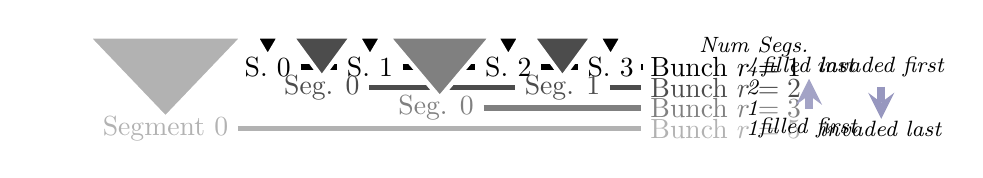
\begin{tikzpicture}[xscale=\X*\linewidth/50cm, yscale=\X*\Y*\linewidth/50cm]
  \begin{scope}
    % Grid
    % \draw[lightgray,step=1] (0,0) grid (50,4);

    % Axes' labels
    % \foreach \x in {1,5,...,49} { \node [below] at (\x,0) {\x}; }
    % \foreach \y in {0,1,...,4} { \node [left] at (0,\y) {\y}; }

\node[anchor=west, text=black!100] (texta) at (24.5, 3.5) {Bunch $r=1$};
\node[anchor=west, text=black!70] (textb) at (24.5, 2.5) {Bunch $r=2$};
\node[anchor=west, text=black!50] (textc) at (24.5, 1.5) {Bunch $r=3$};
\node[anchor=west, text=black!30] (textd) at (24.5, 0.5) {Bunch $r=5$};

\node[anchor=center,font={\footnotesize}] (textx) at (29.2, 4.5) {\textit{Num Segs.}};
\node[anchor=center,font={\footnotesize}] (textax) at (29.2, 3.5) {\textit{4}};
\node[anchor=center,font={\footnotesize}] (textbx) at (29.2, 2.5) {\textit{2}};
\node[anchor=center,font={\footnotesize}] (textcx) at (29.2, 1.5) {\textit{1}};
\node[anchor=center,font={\footnotesize}] (textdx) at (29.2, 0.5) {\textit{1}};

\node[anchor=center,font={\footnotesize}] (textay) at (31.5, 3.5) {\textit{filled last}};
\node[anchor=center,font={\footnotesize}] (textdy) at (31.5, 0.5) {\textit{filled first}};
\draw[-{stealth[scale=0.2]},shorten >=-1mm, shorten <=-0mm, line width=3pt,draw=MidnightBlue!40](textdy.north) -- (textay.south);

\node[anchor=center,font={\footnotesize}] (textay2) at (34.5, 3.5) {\textit{invaded first}};
\node[anchor=center,font={\footnotesize}] (textdy2) at (34.5, 0.5) {\textit{invaded last}};
\draw[-{stealth[scale=0.2]},shorten >=-1mm, shorten <=-0mm, line width=3pt,draw=MidnightBlue!45](textay2.south) -- (textdy2.north);

% Triangles
\filldraw[draw=white,ultra thick,fill=black!100] (8.5,5) -- ++(0.5,-1) -- ++(0.5,1) -- cycle;
\node[anchor=center,text=black!100] (textaa) at (9, 3.5) {S.{} 0};
\filldraw[draw=white,ultra thick,fill=black!100] (12.75,5) -- ++(0.5,-1) -- ++(0.5,1) -- cycle;
\node[anchor=center,text=black!100] (textab) at (13.25, 3.5) {S.{} 1};
\filldraw[draw=white,ultra thick,fill=black!100] (18.5,5) -- ++(0.5,-1) -- ++(0.5,1) -- cycle;
\node[anchor=center,text=black!100] (textac) at (19, 3.5) {S.{} 2};
\filldraw[draw=white,ultra thick,fill=black!100] (22.75,5) -- ++(0.5,-1) -- ++(0.5,1) -- cycle;
\node[anchor=center,text=black!100] (textad) at (23.25, 3.5) {S.{} 3};

% \draw[-stealth, ultra thick, draw=MidnightBlue!80](texta.east) -- (textaa.west);
% \draw[-stealth, ultra thick, draw=MidnightBlue!80](textaa.east) -- (textab.west);
% \draw[-stealth, ultra thick, draw=MidnightBlue!80](textab.east) -- (textac.west);
% \draw[-stealth, ultra thick, draw=MidnightBlue!80](textac.east) -- (textad.west);
\draw[-, line width=2pt, draw=black!100](textaa.east) -- (textab.west);
\draw[-, line width=2pt, draw=black!100](textab.east) -- (textac.west);
\draw[-, line width=2pt, draw=black!100](textac.east) -- (textad.west);
\draw[-, line width=2pt, draw=black!100](textad.east) -- (texta.west);


% Add text
\filldraw[draw=white,ultra thick,fill=black!70] (10,5) -- ++(1.25,-2) -- ++(1.25,2) -- cycle;
\node[anchor=center,text=black!70] (textba) at (11.25, 2.5) {Seg.{} 0};
\filldraw[draw=white,ultra thick,fill=black!70] (20,5) -- ++(1.25,-2) -- ++(1.25,2) -- cycle;
\node[anchor=center,text=black!70] (textbb) at (21.25, 2.5) {Seg.{} 1};


% \draw[-stealth, ultra thick,draw=MidnightBlue!60](textb.east) -- (textba.west);
% \draw[-stealth, ultra thick,draw=MidnightBlue!60](textba.east) -- (textbb.west);
\draw[-,line width=2pt,draw=black!70](textba.east) -- (textbb.west);
\draw[-,line width=2pt,draw=black!70](textbb.east) -- (textb.west);


\filldraw[draw=white,ultra thick,fill=black!50] (14,5) -- ++(2.15,-3) -- ++(2.15,3) -- cycle;
\node[anchor=center,text=black!50] (textca) at (16, 1.5) {Seg.{} 0};

% \draw[-stealth, ultra thick,draw=MidnightBlue!40](textc.east) -- (textca.west);
\draw[-, line width=2pt,draw=black!50](textca.east) -- (textc.west);

\filldraw[draw=white,ultra thick,fill=black!30] (1.5,5) -- ++(3.25,-4) -- ++(3.25,4) -- cycle;
\node[anchor=center,text=black!30] (textda) at (4.75, 0.5) {Segment{} 0};

% \draw[-stealth, ultra thick,draw=MidnightBlue!20](textd.east) -- (textda.west);
\draw[-, line width=2pt,draw=black!30](textda.east) -- (textd.west);


\node[anchor=west] (textbunch) at (-1, 4.2) {\phantom{Bunch}};
  % \draw [draw=MidnightBlue!30, -to, very ultra thick, shorten >=0.5mm] (textd.west) to[out=180, in=215, looseness=1.5] (textc.west);
  % \draw [draw=MidnightBlue!50, -to, very ultra thick, shorten >=0.5mm] (textc.west) to[out=180, in=215, looseness=1.5] (textb.west);
  % \draw [draw=MidnightBlue!70, -to, very ultra thick] (textb.west) to[out=180, in=215, looseness=1.5] (texta.west);

% \filldraw[draw=white,ultra thick,fill=black!100] (23+8.5,5) -- ++(0.5,-1) -- ++(0.5,1) -- cycle;
% \filldraw[draw=white,ultra thick,fill=black!100] (23+12.75,5) -- ++(0.5,-1) -- ++(0.5,1) -- cycle;
% \filldraw[draw=white,ultra thick,fill=black!100] (23+18.5,5) -- ++(0.5,-1) -- ++(0.5,1) -- cycle;
% \filldraw[draw=white,ultra thick,fill=black!100] (23+22.75,5) -- ++(0.5,-1) -- ++(0.5,1) -- cycle;
% \filldraw[draw=white,ultra thick,fill=black!70] (23+10,5) -- ++(1.25,-2) -- ++(1.25,2) -- cycle;
% \filldraw[draw=white,ultra thick,fill=black!70] (23+20,5) -- ++(1.25,-2) -- ++(1.25,2) -- cycle;
% \filldraw[draw=white,ultra thick,fill=black!25] (23+14,5) -- ++(2.15,-3) -- ++(2.15,3) -- cycle;
% \filldraw[draw=white,ultra thick,fill=black!10] (23+1.5,5) -- ++(3.25,-4) -- ++(3.25,4) -- cycle;

  \end{scope}
\end{tikzpicture}
\end{subfigure}

\begin{subfigure}{0.5\textwidth}
\scalebox{\X}{%
\includegraphics[width=\textwidth, clip, trim={0 0 1.25cm 11.2cm}]%
{binder-20a-tilted-eulerian-surface/binder/teeplots/20a/color-epoch-t=black+color-metaepoch-tau=black+color-site-k=black+font.family=serif+plotter=site_reservation_size_at_rank_heatmap+surface-size=16+swap-yaxes=True+symbol-color=black+viz=site-reservation.../-at-ranks-heatmap+ext=.pdf}%
}\vspace{-1ex}
\end{subfigure}%
\begin{subfigure}{0.5\textwidth}~\end{subfigure}\vspace{-1ex}

\vspace{-1.5ex}

\caption{
    \textbf{Storage layout detail.}
    \footnotesize
    Epoch-by-epoch storage layout of \hv{} reservation ``segments''  for buffer size $S=16$, shown as contiguous horizontal regions divided by solid black line; time from bottom to top.
    Segments are categorized into ``bunches'' according to their initial size $r$.
    Inverted triangles schematize the layout of segment bunches, which are nested and discontiguous.
    As epochs elapse, segments grow from initial size $r$ to mature size $R$ and are then ``invaded'' to elimination by growth of their left neighbor.
    (For bunch $r=1$, $R=1$; for bunch $r=2$, $R=3$, etc.)
    Because the segment sizes $r$ mirror the hanoi sequence, expansion of invading segments by one site per epoch ensures buffer space for instances of high \hv{} as they are encountered at later $\colorT$ (see Figure \ref{fig:hanoi-intuition}).
  }
  \label{fig:hsurf-stretched-intuition}
\end{figure*}
